% !TeX root = main.tex
\newpage
\clearpage
\subsection{Particle-Boundary Resolution} \label{pbh}

\Figo{InventortCDN} illustrates the CD nozzle modeled in this application. When displayed in the application it is a facade to provide the viewer a sense of proportions. 

\begin{figure}[H]
\centering
\includegraphics[width=5.10in]{../images/InventortCDN.png}
\captionof{figure}[Dobule Cone]{\textit{Actual Converging-Diverging Nozzel design.}}
\label{fig:InventortCDN}
\end{figure}


\Figo{InventortCDNDWG} shows the actual dimension of the CD nozzle. It has a very wide throat so to to insure low density flow. The measures are dimensionless and can be mm, cm, etc. 
\begin{figure}[H]
\centering
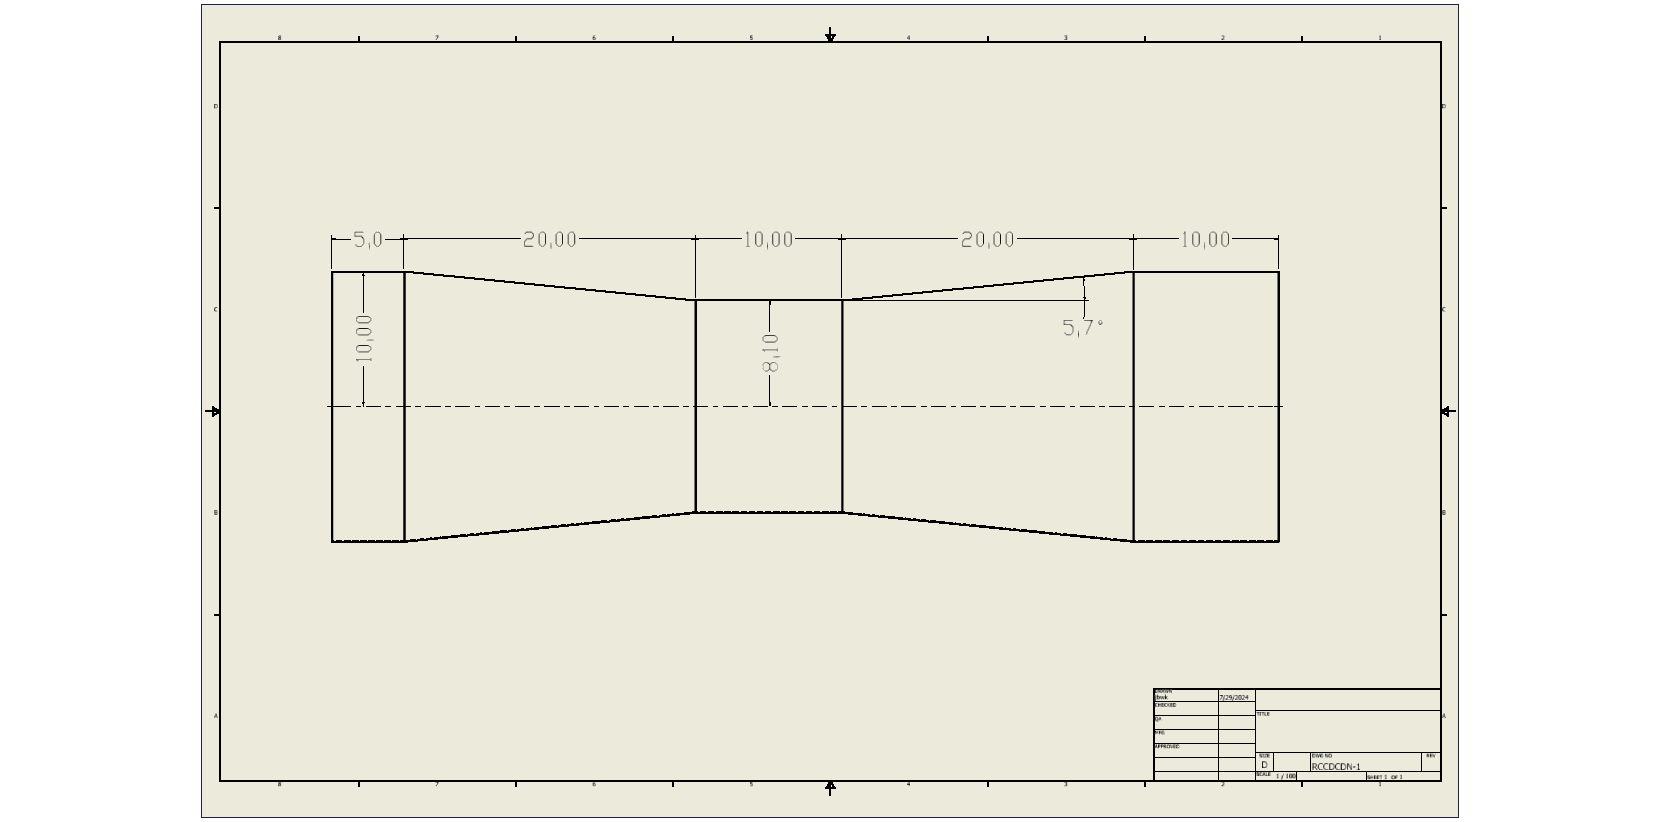
\includegraphics[width=6.80in]{../images/InventortCDNDWG.png}
\captionof{figure}[Dobule Cone]{\textit{Converging-Diverging Nozzel design specifications.}}
\label{fig:InventortCDNDWG}
\end{figure}


A number of Matlab applications were developed to analyze and debug logic. \Figo{RCCDBoundaryWhole} shows the plot of the CD nozzle with points of intersection on the tangent plane. 
Fig. \ref{fig:RCCDBoundaryWhole}
\input{../images/RCCDBoundaryWhole.tex}

The challenge in boundary calculations is to establish the plane tangent to the boundary at the point of contact. This requires the establishment of three independent vectors terminating in the plane. Once the tangent plane is formed the normal vector is determined and the collision reaction is calculated by reflecting the particle around it. 

The black asterisk represents point A ($P_a$), at the same angle as the particle, but at the radius of the boundary. The blue point B ($P_b$), represents a point at the same angle as the particle, but down the length of the nozzle at a lower radius. The red point C ($P_c$), represents a point at the same radius as point B but at a slightly different angle and therefore parallel to it. These three points constitute independent vectors terminating on a plane tangent to the slope of the nozzle at that point. From these points the normal of the tangent plane is calculated, $\vec{N}$, which is the mauve dotted line. The green vector is the incoming velocity ($V_{in}$), which is reflected around the normal to produce the output velocity ($V_{out}$), represented by the yellow line.
\input{../images/RCCDBoundaryCPoint.tex}

Where the boundary is flat the negative of the \textit{xy} components of velocity are taken. When the three independent points are found the unit normal is calculated according to (\ref{eqn:bound001}).
\begin{equation}
 \begin{aligned}
 \hat{N}=\frac{\left(\vec{P_a}-\vec{P_b}\right)\otimes\left(\vec{P_a}-\vec{P_c}\right)}{||\vec{N}||}\label{eqn:bound001} 
\end{aligned}
\end{equation}


With the unit normal in hand the reflected velocity out, ($\vec{V_{out}}$) is determined by (\ref{eqn:bound002}) 
\begin{equation}
 \begin{aligned}
 \vec{V_{out}} = \vec{V_{in}} - 2.0(\vec{V_{in}}\bullet\hat{N})\hat{N}\label{eqn:bound002} 
\end{aligned}
\end{equation}


Boundary particles are placed in every cell which contains a portion of the boundary. Fig. \ref{fig:CDNozBoundaryCellSlice} shows a slice of the CDN with the boundary in black and boundary particles in red. Notice that there is a red particle in every cell through which the boundary travels. 
\input{../images/CDNozBoundaryCellSlice.tex}

Fig. \ref{fig:CDNozBoundaryAll} shows the complete nozzle with all the boundary particles in place.

Processing boundaries in this manner means that a particle will only check for a boundary if it is in a cell with one - this saves calculating boundary proximity for every particle every frame. 
Boundary particles are convenient in another manner. Notice that the equation (\ref{eqn:bound001}) requires a normalized normal vector which in turn requires a square root. If the range of boundary that passes through the cell is considered infinitesimal, then the unit normal can be calculated and stored on the CPU before transfer to the GPU. This is a concept borrowed from computer graphics where normals are sent with triangle primitives. 


The process of boundary collision resolution is a little bit more complicated. \Figo{ProcessCDNBoundary} shows the code for processing the boundary. It begins by insuring boundary particles are not considered since they are stationary. When the simulation setup is performed the boundary particles are added first, then the actual particles. Any particle number greater than the last boundary particle is then an moving particle. 

\input{../images/CDNozBoundaryAll.tex}


The \textit{active location} of the boundary is stored in the boundary particle velocity components. In this case they will all be non-zero if it is a particle boundary. 

But, imagine a cube with boundary particles. If the boundary lay in the middle of a cube wall then the only location that will have a collision will be the single dimension. In a particle is in the corner of the cube the particle can reflect off of three sides. In this case, the three velocity components will be nonzero.
\begin{figure}[H]
\centering
\includegraphics[width=2.97in]{../imgperm/SimpleConfig.png}
\captionof{figure}[Dobule Cone]{\textit{The setup for a simple demonstration. The particles in blue are arranged at the top and bottom of the starting point of the nozzle and aimed at the sloping sections.}}
\label{fig:SimpleConfig}
\end{figure}



The code for particle-boundary collisions is detailed in the Appendix section \ref{ppcrc}

\begin{figure}
\centering
\lstset{style=gpucode,linewidth=6.5in,xleftmargin=0.25in}

\begin{lstlisting}
index = 0;
Sidelen = 64;
PipeCenter = 11.0000;
PipeRadius = 10.0000;
CellAryW = 20;
CellAryH = 20;
CellAryL = 64;
radius = 0.2;
PartPerCell = 8;
pcount = 5304;
colcount = 0;
dataFile = "J:/RCCDData/perfdataM/CDNozBoundaryTest.bin";
aprFile = "J:/RCCDData/perfdataM/CDNozBoundaryTest.csv";
density = 0.0;
pdensity = 0.0;
dispatchx =  5305;
dispatchy = 1;
dispatchz = 1;
workGroupsx = 1;
workGroupsy = 1;
workGroupsz = 1;
ColArySize = 128;
MaxSingleCollisions = 8;

\end{lstlisting}


\caption[Benchset test configuration file]{The benchset test configuration file provides information on each test to be run by \app{} }
\label{fig:tstfile}
\end{figure}






